\documentclass[border=4pt]{standalone}
\usepackage{tikz}
\usetikzlibrary{positioning, arrows.meta, calc, fit, backgrounds}
\usepackage{amsmath,amssymb}
\begin{document}
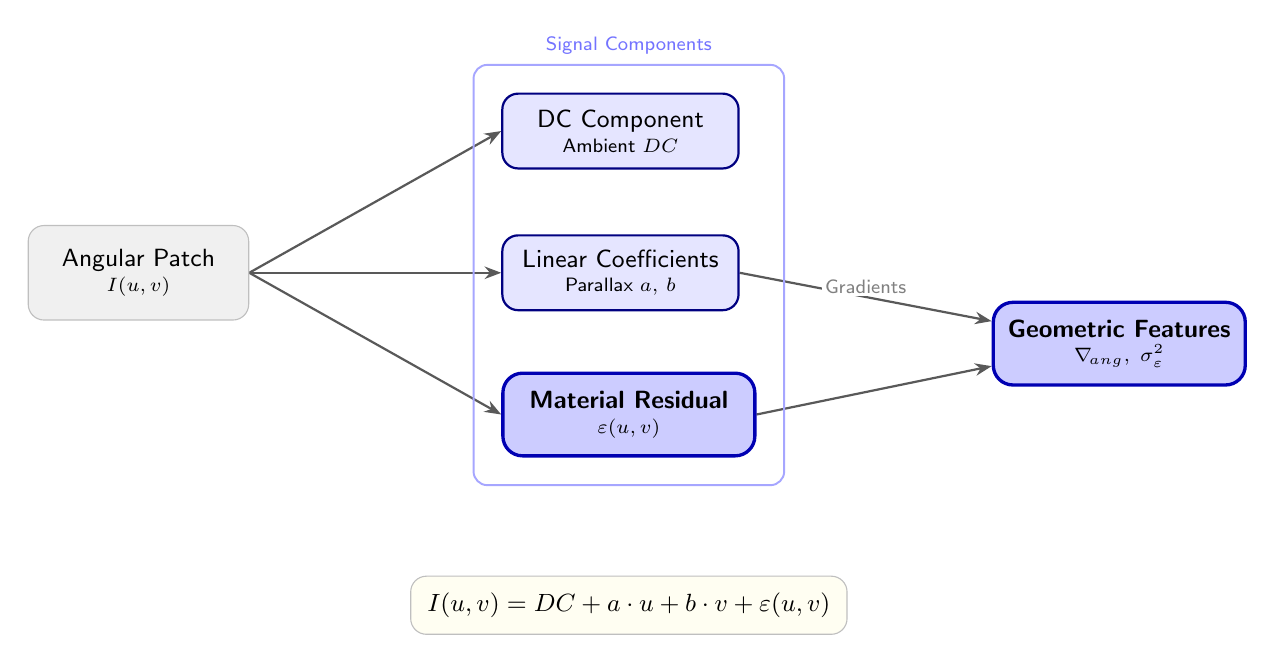
\begin{tikzpicture}[
  input/.style={draw, rounded corners=2mm, minimum width=2.8cm, minimum height=1.2cm,
                fill=gray!12, draw=gray!50, align=center, font=\sffamily\small},
  module/.style={draw, rounded corners=2mm, minimum width=3.0cm, minimum height=0.95cm,
                 fill=blue!10, draw=blue!50!black, line width=0.8pt, align=center,
                 font=\sffamily\small},
  innov/.style={draw, rounded corners=2.5mm, minimum width=3.2cm, minimum height=1.05cm,
                fill=blue!20, draw=blue!70!black, line width=1.2pt, align=center,
                font=\sffamily\small\bfseries},
  arr/.style={-{Stealth[length=6pt]}, thick, color=black!65},
  arrlbl/.style={font=\sffamily\scriptsize, text=black!50, fill=white, inner sep=1pt},
  gbox/.style={draw=blue!35, rounded corners=5pt, inner sep=10pt, line width=0.7pt},
  lbl/.style={font=\sffamily\scriptsize, text=blue!55},
  eqbox/.style={draw=black!25, rounded corners=2mm, fill=yellow!5, inner sep=6pt,
                font=\small},
]

% Input
\node[input] (m1) {Angular Patch\\[-2pt]{\scriptsize $I(u,v)$}};

% Signal decomposition outputs (middle column)
\node[module, right=3.2cm of m1, yshift=1.8cm] (m2)
  {DC Component\\[-2pt]{\scriptsize Ambient $DC$}};
\node[module, right=3.2cm of m1] (m3)
  {Linear Coefficients\\[-2pt]{\scriptsize Parallax $a,\, b$}};
\node[innov, right=3.2cm of m1, yshift=-1.8cm] (m4)
  {\textbf{Material Residual}\\[-2pt]{\scriptsize $\varepsilon(u,v)$}};

% Output (right column)
\node[innov, right=3.2cm of m3, yshift=-0.9cm] (m5)
  {\textbf{Geometric Features}\\[-2pt]{\scriptsize $\nabla_{\!ang},\;\sigma_\varepsilon^{2}$}};

% Arrows
\begin{scope}[on background layer]
  \draw[arr] (m1.east) -- (m2.west);
  \draw[arr] (m1.east) -- (m3.west);
  \draw[arr] (m1.east) -- (m4.west);
  \draw[arr] (m3.east) -- node[arrlbl, above] {Gradients} (m5.170);
  \draw[arr] (m4.east) -- (m5.190);
\end{scope}

% Group box
\node[gbox, fit=(m2)(m3)(m4),
      label={[lbl]above:Signal Components}] {};

% Equation annotation
\node[eqbox, below=1.5cm of m4]
  {$I(u,v) = DC + a \cdot u + b \cdot v + \varepsilon(u,v)$};

\end{tikzpicture}
\end{document}